\section{Benutzeroberfl\"ache}

Beim Starten der Applikation \"offnet sich das User Interface des Simulators auf dem die Funktionen des PICs nachvollzogen werden k\"onnen.

\begin{figure}[h]
\centering
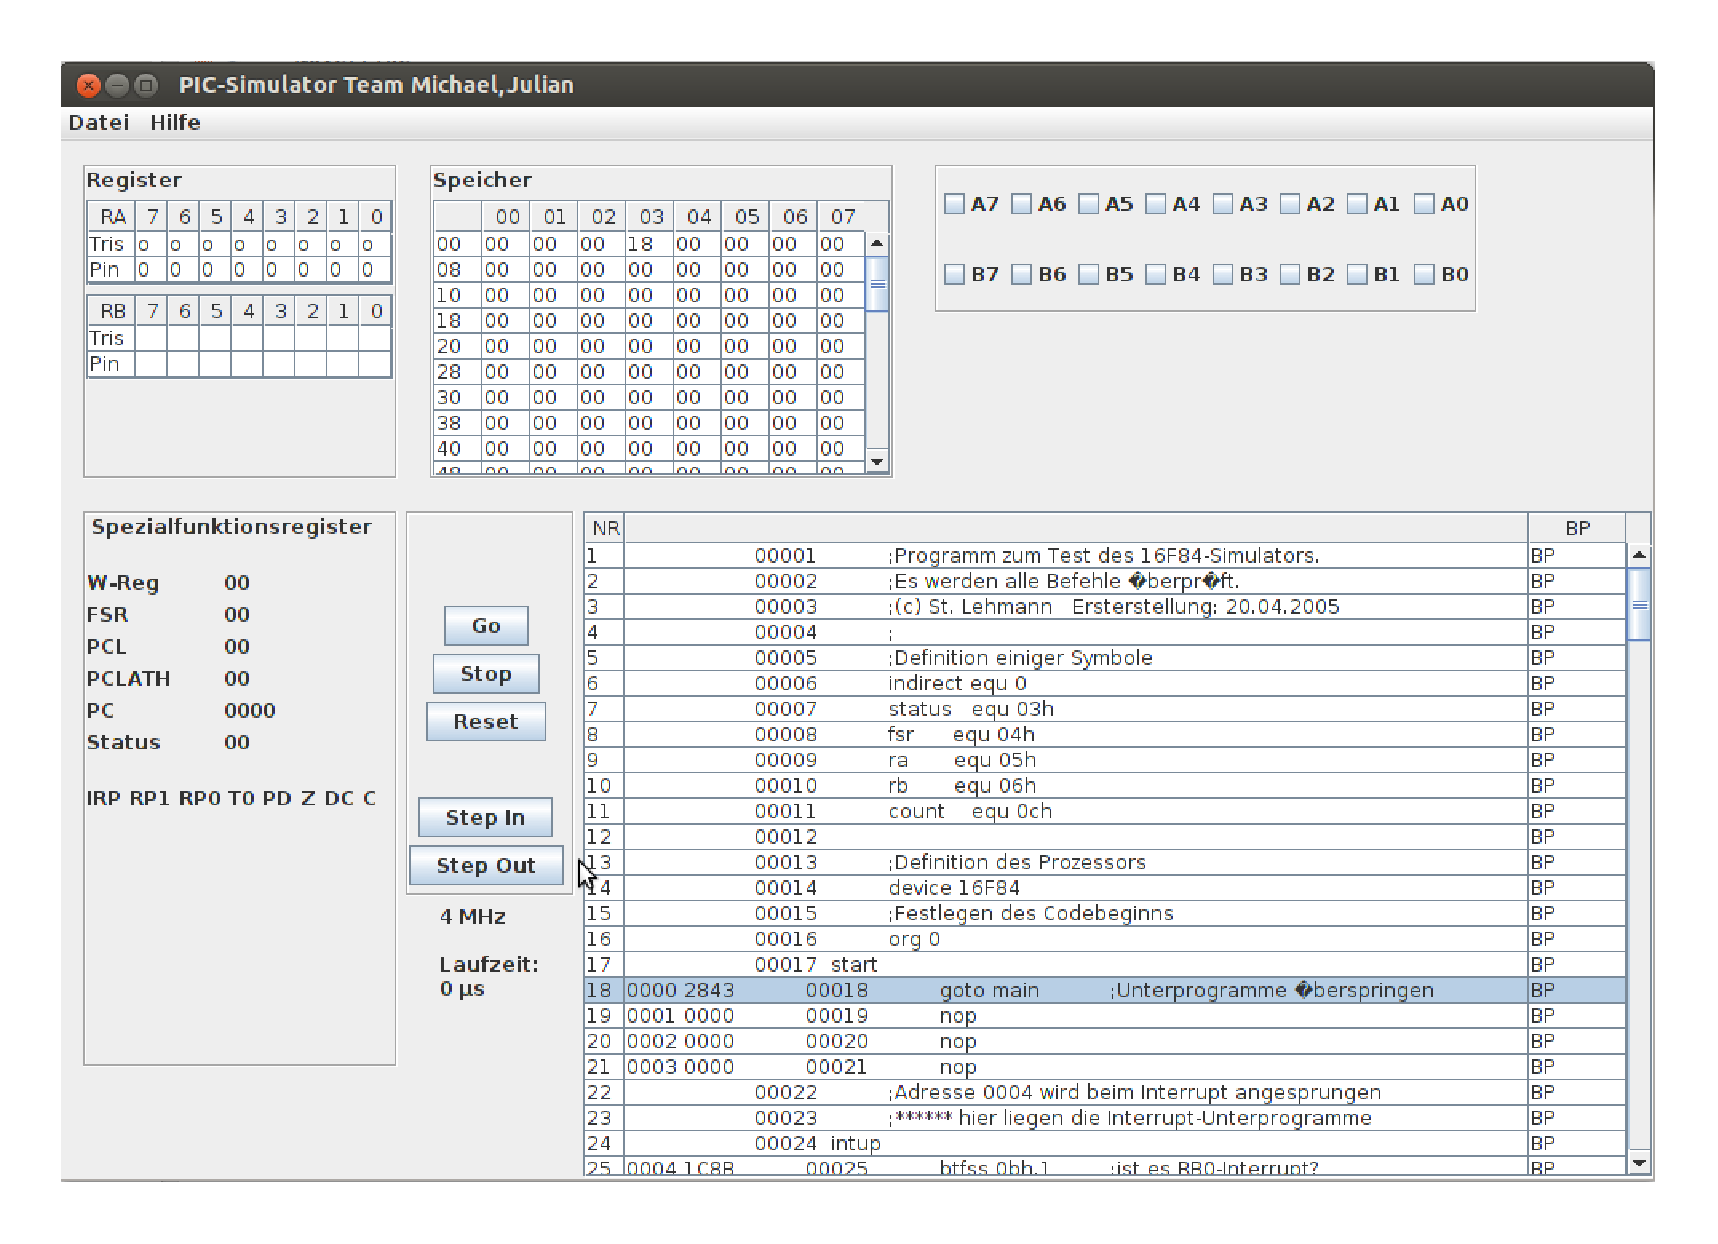
\includegraphics[scale=0.4]{Bilder/GUI.pdf}
\caption{GUI}
\end{figure}
\newpage

\noindent \"Uber „Datei“ und „Datei \"offnen“ lassen sich Quellcode-Dateien \"offnen. In die Dateiauswahl ist ein Dateifilter integriert der ausschließlich .LST-Dateien anzeigt.

\begin{figure}[h]
\centering
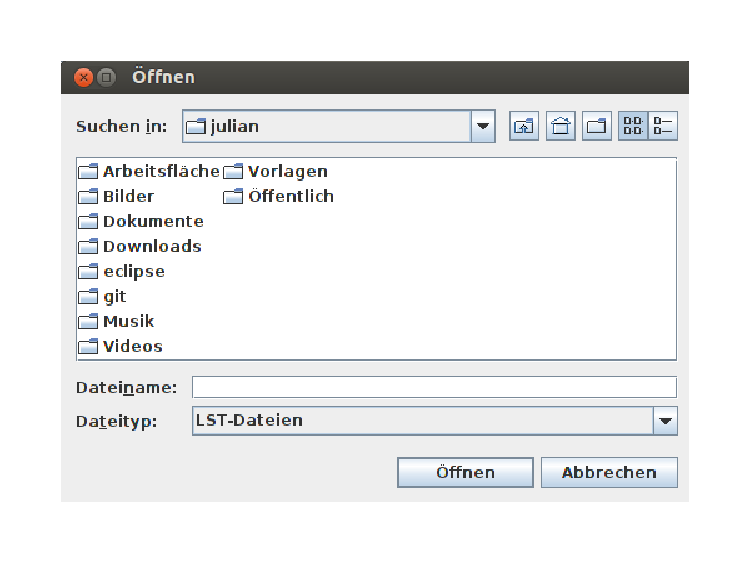
\includegraphics[scale=0.7]{Bilder/Offnen.pdf}
\caption{Datei \"offnen}
\end{figure}

\noindent Mit den Buttons \glqq Step-In\grqq , \glqq Step-Out\grqq , \glqq Go\grqq , \glqq Stop\grqq  und \glqq Reset\grqq  l\"asst sich der Simulationsablauf steuern. Mit Step-In und Step-Out l\"asst sich jeweils nur ein Programmschritt ausf\"uhren, mit Go wird das Programm komplett abgearbeitet. Mit Stop stoppt der Simulationsvorgang und mit Reset wird er komplett zur\"uckgesetzt.

\begin{figure}[h]
\centering
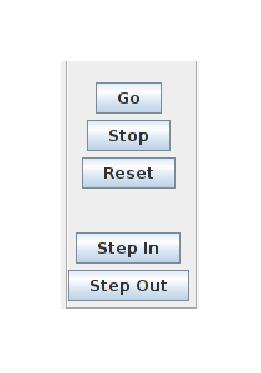
\includegraphics[scale=0.5]{Bilder/Buttons.pdf}
\caption{Kontroll-Buttons}
\end{figure}

Die Register werden in der linken oberen Ecke des User Interfaces angezeigt. Die werte des Spezialfunktionsregister wird darunter dargestellt. Die  Darstellung der Werte erfolgt im Hexadezimalsystem.

\begin{figure}[h]
\centering
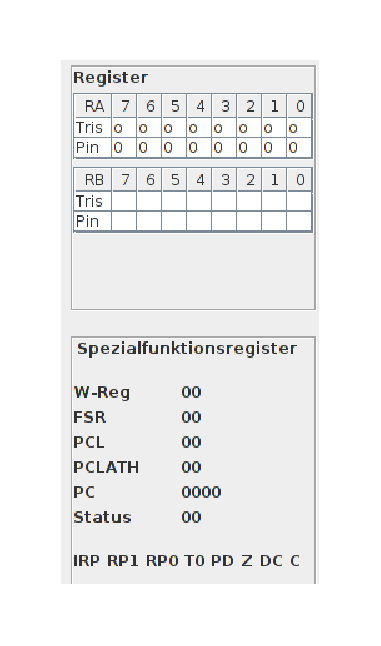
\includegraphics[scale=0.5]{Bilder/Register.pdf}
\caption{Register und Spezialfunktionsregister}
\end{figure}

Die Speicherinhalte werden in Form einer Tabelle am oberen Rand des User Interfaces dargestellt. Die Werte werden im Hexadezimalsystem wiedergegeben. 


\noindent In der rechten unteren Ecke wir der Quelltext des zu simulierenden Programmes angezeigt. Dieser wir wie beschrieben \"uber \glqq Datei \"offnen\grqq in die Tabelle geschrieben.

\begin{figure}[h]
\centering
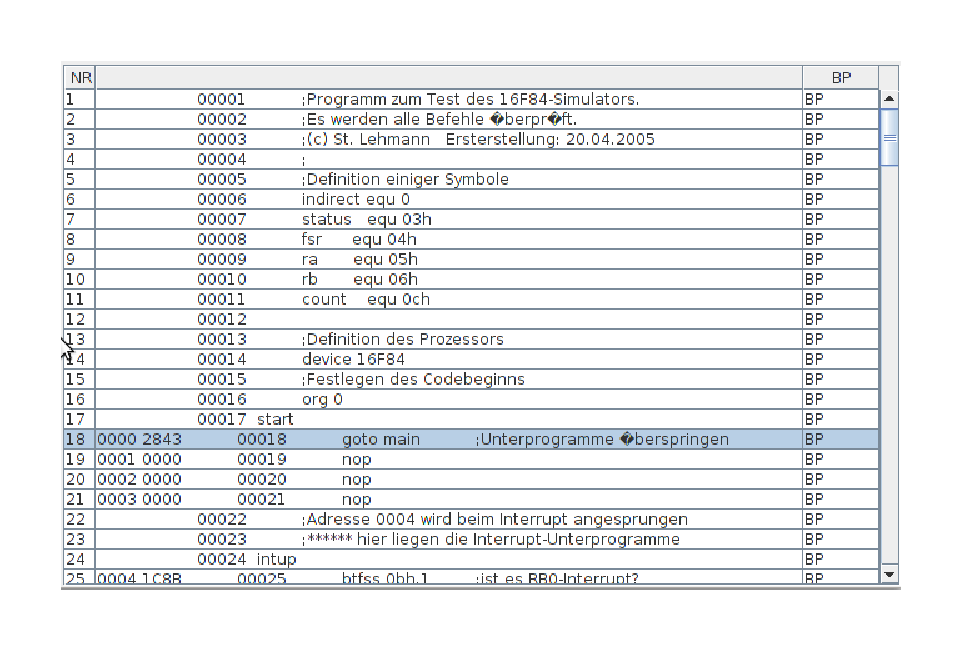
\includegraphics[scale=0.5]{Bilder/Text.pdf}
\caption{Textfeld f\"ur den Quelltext}
\end{figure}